
\documentclass[letterpaper,hide notes,xcolor={table,svgnames},pdftex,10pt]{beamer}
\def\showexamples{t}


%\usepackage[svgnames]{xcolor}

%% Demo talk
%\documentclass[letterpaper,notes=show]{beamer}

\usecolortheme{crane}
\setbeamertemplate{navigation symbols}{}

\usetheme{MyPittsburgh}
%\usetheme{Frankfurt}

%\usepackage{tipa}

\usepackage{hyperref}
\usepackage{graphicx,xspace}
\usepackage[normalem]{ulem}
\usepackage{multicol}

\newcommand\SF[1]{$\bigstar$\footnote{SF: #1}}

\usepackage[default]{sourcesanspro}
\usepackage[T1]{fontenc}

\newcounter{tmpnumSlide}
\newcounter{tmpnumNote}

% old question code
%\newcommand\question[1]{{$\bigstar$ \small \onlySlide{2}{#1}}}
% \newcommand\nquestion[1]{\ifdefined \presentationonly \textcircled{?} \fi \note{\par{\Large \textbf{?}} #1}}
% \newcommand\nanswer[1]{\note{\par{\Large \textbf{A}} #1}}


 \newcommand\mnote[1]{%
   \addtocounter{tmpnumSlide}{1}
   \ifdefined\showcues {~\tiny\fbox{\arabic{tmpnumSlide}}}\fi
   \note{\setlength{\parskip}{1ex}\addtocounter{tmpnumNote}{1}\textbf{\Large \arabic{tmpnumNote}:} {#1\par}}}

\newcommand\mmnote[1]{\note{\setlength{\parskip}{1ex}#1\par}}

%\newcommand\mnote[2][]{\ifdefined\handoutwithnotes {~\tiny\fbox{#1}}\fi
% \note{\setlength{\parskip}{1ex}\textbf{\Large #1:} #2\par}}

%\newcommand\mnote[2][]{{\tiny\fbox{#1}} \note{\setlength{\parskip}{1ex}\textbf{\Large #1:} #2\par}}

\newcommand\mquestion[2]{{~\color{red}\fbox{?}}\note{\setlength{\parskip}{1ex}\par{\Large \textbf{?}} #1} \note{\setlength{\parskip}{1ex}\par{\Large \textbf{A}} #2\par}\ifdefined \presentationonly \pause \fi}

\newcommand\blackboard[1]{%
\ifdefined   \showblackboard
  {#1}
  \else {\begin{center} \fbox{\colorbox{blue!30}{%
         \begin{minipage}{.95\linewidth}%
           \hspace{\stretch{1}} Some space intentionally left blank; done at the blackboard.%
         \end{minipage}}}\end{center}}%
         \fi%
}



%\newcommand\q{\tikz \node[thick,color=black,shape=circle]{?};}
%\newcommand\q{\ifdefined \presentationonly \textcircled{?} \fi}

\usepackage{listings}
\lstset{%
  keywordstyle=\bfseries,
  aboveskip=15pt,
  belowskip=15pt,
  captionpos=b,
  identifierstyle=\ttfamily,
  escapeinside={(*@}{@*)},
  stringstyle=\ttfamiliy,
  frame=lines,
  numbers=left, basicstyle=\scriptsize, numberstyle=\tiny, stepnumber=0, numbersep=2pt}

\usepackage{siunitx}
\newcommand\sius[1]{\num[group-separator = {,}]{#1}\si{\micro\second}}
\newcommand\sims[1]{\num[group-separator = {,}]{#1}\si{\milli\second}}
\newcommand\sins[1]{\num[group-separator = {,}]{#1}\si{\nano\second}}
\sisetup{group-separator = {,}, group-digits = true}

%% -------------------- tikz --------------------
\usepackage{tikz}
\usetikzlibrary{positioning}
\usetikzlibrary{arrows,backgrounds,automata,decorations.shapes,decorations.pathmorphing,decorations.markings,decorations.text}

\tikzstyle{place}=[circle,draw=blue!50,fill=blue!20,thick, inner sep=0pt,minimum size=6mm]
\tikzstyle{transition}=[rectangle,draw=black!50,fill=black!20,thick, inner sep=0pt,minimum size=4mm]

\tikzstyle{block}=[rectangle,draw=black, thick, inner sep=5pt]
\tikzstyle{bullet}=[circle,draw=black, fill=black, thin, inner sep=2pt]

\tikzstyle{pre}=[<-,shorten <=1pt,>=stealth',semithick]
\tikzstyle{post}=[->,shorten >=1pt,>=stealth',semithick]
\tikzstyle{bi}=[<->,shorten >=1pt,shorten <=1pt, >=stealth',semithick]

\tikzstyle{mut}=[-,>=stealth',semithick]

\tikzstyle{treereset}=[dashed,->, shorten >=1pt,>=stealth',thin]

\usepackage{ifmtarg}
\usepackage{xifthen}
\makeatletter
% new counter to now which frame it is within the sequence
\newcounter{multiframecounter}
% initialize buffer for previously used frame title
\gdef\lastframetitle{\textit{undefined}}
% new environment for a multi-frame
\newenvironment{multiframe}[1][]{%
\ifthenelse{\isempty{#1}}{%
% if no frame title was set via optional parameter,
% only increase sequence counter by 1
\addtocounter{multiframecounter}{1}%
}{%
% new frame title has been provided, thus
% reset sequence counter to 1 and buffer frame title for later use
\setcounter{multiframecounter}{1}%
\gdef\lastframetitle{#1}%
}%
% start conventional frame environment and
% automatically set frame title followed by sequence counter
\begin{frame}%
\frametitle{\lastframetitle~{\normalfont(\arabic{multiframecounter})}}%
}{%
\end{frame}%
}
\makeatother

\makeatletter
\newdimen\tu@tmpa%
\newdimen\ydiffl%
\newdimen\xdiffl%
\newcommand\ydiff[2]{%
    \coordinate (tmpnamea) at (#1);%
    \coordinate (tmpnameb) at (#2);%
    \pgfextracty{\tu@tmpa}{\pgfpointanchor{tmpnamea}{center}}%
    \pgfextracty{\ydiffl}{\pgfpointanchor{tmpnameb}{center}}%
    \advance\ydiffl by -\tu@tmpa%
}
\newcommand\xdiff[2]{%
    \coordinate (tmpnamea) at (#1);%
    \coordinate (tmpnameb) at (#2);%
    \pgfextractx{\tu@tmpa}{\pgfpointanchor{tmpnamea}{center}}%
    \pgfextractx{\xdiffl}{\pgfpointanchor{tmpnameb}{center}}%
    \advance\xdiffl by -\tu@tmpa%
}
\makeatother
\newcommand{\copyrightbox}[3][r]{%
\begin{tikzpicture}%
\node[inner sep=0pt,minimum size=2em](ciimage){#2};
\usefont{OT1}{phv}{n}{n}\fontsize{4}{4}\selectfont
\ydiff{ciimage.south}{ciimage.north}
\xdiff{ciimage.west}{ciimage.east}
\ifthenelse{\equal{#1}{r}}{%
\node[inner sep=0pt,right=1ex of ciimage.south east,anchor=north west,rotate=90]%
{\raggedleft\color{black!50}\parbox{\the\ydiffl}{\raggedright{}#3}};%
}{%
\ifthenelse{\equal{#1}{l}}{%
\node[inner sep=0pt,right=1ex of ciimage.south west,anchor=south west,rotate=90]%
{\raggedleft\color{black!50}\parbox{\the\ydiffl}{\raggedright{}#3}};%
}{%
\node[inner sep=0pt,below=1ex of ciimage.south west,anchor=north west]%
{\raggedleft\color{black!50}\parbox{\the\xdiffl}{\raggedright{}#3}};%
}
}
\end{tikzpicture}
}


%% --------------------

%\usepackage[excludeor]{everyhook}
%\PushPreHook{par}{\setbox0=\lastbox\llap{MUH}}\box0}

%\vspace*{\stretch{1}

%\setbox0=\lastbox \llap{\textbullet\enskip}\box0}

\setlength{\parskip}{\fill}

\newcommand\noskips{\setlength{\parskip}{1ex}}
\newcommand\doskips{\setlength{\parskip}{\fill}}

\newcommand\xx{\par\vspace*{\stretch{1}}\par}
\newcommand\xxs{\par\vspace*{2ex}\par}
\newcommand\tuple[1]{\langle #1 \rangle}
\newcommand\code[1]{{\sf \footnotesize #1}}
\newcommand\ex[1]{\uline{Example:} \ifdefined \presentationonly \pause \fi
  \ifdefined\showexamples#1\xspace\else{\uline{\hspace*{2cm}}}\fi}

\newcommand\ceil[1]{\lceil #1 \rceil}


\AtBeginSection[]
{
   \begin{frame}
       \frametitle{Outline}
       \tableofcontents[currentsection]
   \end{frame}
}



\pgfdeclarelayer{edgelayer}
\pgfdeclarelayer{nodelayer}
\pgfsetlayers{edgelayer,nodelayer,main}

\tikzstyle{none}=[inner sep=0pt]
\tikzstyle{rn}=[circle,fill=Red,draw=Black,line width=0.8 pt]
\tikzstyle{gn}=[circle,fill=Lime,draw=Black,line width=0.8 pt]
\tikzstyle{yn}=[circle,fill=Yellow,draw=Black,line width=0.8 pt]
\tikzstyle{empty}=[circle,fill=White,draw=Black]
\tikzstyle{bw} = [rectangle, draw, fill=blue!20, 
    text width=4em, text centered, rounded corners, minimum height=2em]
    
    \newcommand{\CcNote}[1]{% longname
	This work is licensed under the \textit{Creative Commons #1 3.0 License}.%
}
\newcommand{\CcImageBy}[1]{%
	\includegraphics[scale=#1]{creative_commons/cc_by_30.pdf}%
}
\newcommand{\CcImageSa}[1]{%
	\includegraphics[scale=#1]{creative_commons/cc_sa_30.pdf}%
}
\newcommand{\CcImageNc}[1]{%
	\includegraphics[scale=#1]{creative_commons/cc_nc_30.pdf}%
}
\newcommand{\CcGroupBySa}[2]{% zoom, gap
	\CcImageBy{#1}\hspace*{#2}\CcImageNc{#1}\hspace*{#2}\CcImageSa{#1}%
}
\newcommand{\CcLongnameByNcSa}{Attribution-NonCommercial-ShareAlike}

\newenvironment{changemargin}[1]{% 
  \begin{list}{}{% 
    \setlength{\topsep}{0pt}% 
    \setlength{\leftmargin}{#1}% 
    \setlength{\rightmargin}{1em}
    \setlength{\listparindent}{\parindent}% 
    \setlength{\itemindent}{\parindent}% 
    \setlength{\parsep}{\parskip}% 
  }% 
  \item[]}{\end{list}} 




\title{Lecture 21 --- Business \& Employment Equity }

\author{Jeff Zarnett, based on original by Douglas Harder \\ \small \texttt{jzarnett@uwaterloo.ca} / \texttt{dwharder@uwaterloo.ca}}
\institute{Department of Electrical and Computer Engineering \\
  University of Waterloo}
\date{\today}


\begin{document}

\begin{frame}
  \titlepage

\begin{center}
  \small{Acknowledgments: Douglas Harder~\cite{dwh}, Julie Vale~\cite{jv}}
  \end{center}
\end{frame}

\part{Forms of Business}

\begin{frame}
\partpage
\end{frame}



\begin{frame}
\frametitle{Mind Your Business}

Business, \textit{n}:\\
\quad Trade and all activity relating to it, especially considered in terms of volume or profitability; commercial transactions, engagements, and undertakings regarded collectively; an instance of this.

Hence more generally: the world of trade and commerce.

Reference:  Oxford English Dictionary (www.oed.com)

\end{frame}



\begin{frame}
\frametitle{Forms of Business}

There are three main ways to organize a business:

\begin{itemize}
	\item Sole proprietorship
	\item Partnership
	\item Corporation
\end{itemize}

\end{frame}



\begin{frame}
\frametitle{Sole Proprietorship}

In a sole proprietorship, the business is owned and operated by a natural person (human).

This individual may employ others in pursuit of his or her business.

There is no legal distinction between the owner and the business.

The trade or business name, need not be his or her legal name.

The owner receives all profits and has unlimited responsibility for all risks including loses and debts.

All assets of the business are owned by the owner.

What are the advantages and disadvantages of this structure?

\end{frame}



\begin{frame}
\frametitle{Sole Proprietorship}

Advantages:\\
\quad Minimal government regulation\\
\quad The owner has control over all the business

Disadvantages:\\
\quad It is difficult to raise capital\\
\quad The owner's illness may affect the business significantly

\end{frame}



\begin{frame}
\frametitle{Partnership}

A partnership is a business between two or more legal persons.

The partnership may employ others in pursuit of its business.

The profits and risks (losses and debts) are now shared between the partners.

\end{frame}



\begin{frame}
\frametitle{Partnership}

In Canada, partnerships are governed by the Partnerships Act, Ontario:

\begin{quote}
Partnership is the relation that subsists between persons carrying on a business in common with a view to profit
\end{quote}

The determination of a partnership is a matter of common law which interprets the clause:

\begin{quote}
The receipt by a person of a share of the profits of a business
   is proof, in the absence of evidence to the contrary, that the
   person is a partner in the business.
\end{quote}

\end{frame}



\begin{frame}
\frametitle{The Buck Stops Here}

The Act defines a firm as all persons who have entered into partnership with one another.

If one partner commits an illegal act, all partners are liable for any consequences.

In some cases, partners can choose to have limited liability; however, they may have restricted control over the actions of the partnership.

At least 1 partner must assume liability for the losses/debts of the partnership.


\end{frame}



\begin{frame}
\frametitle{In-cor-po-raaaaaaate!}

A Corporation is a separate legal entity that one creates by filing the paperwork. 

It allows limited liability: shareholders of the corporation are not responsible for its debts (unless they provide personal guarantees)...

Unless, of course, the shareholder is also a director...!

There are also tax benefits and better access to capital and grants. 

\end{frame}



\begin{frame}
\frametitle{Corporation}

But this also comes with costs: the costs to file, administrative work (articles, returns, corporate income tax returns, etc etc.)

A corporation has a complex structure:
\begin{itemize}
	\item Shareholders - owners of the corporation.
	\item Directors - the manager(s) of the corporation.
	\item Officers - people with specific roles (CEO, president, etc.)
\end{itemize}

Individuals may have multiple roles.

\end{frame}



\begin{frame}
\frametitle{Bankruptcy}

\begin{center}
	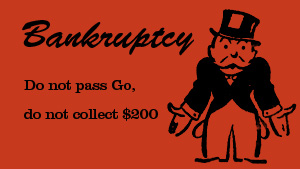
\includegraphics{images/Bankruptcy_monopoly.jpg}
\end{center}

(Source: From the board game ``Monopoly'')

\end{frame}



\begin{frame}
\frametitle{Insolvency}

When a legal person cannot repay its debts to creditors, it is said to be insolvent.

This may include:\\
\quad \alert{Cash flow insolvency}, the inability to pay short-term obligations.\\
\quad \alert{Balance sheet insolvency}, where liabilities exceed assets.
	
	A legal person may be one without being the other, but in the case where one is in both, the person is said to be in a state of bankruptcy.

\end{frame}

\part{Employment Equity}

\begin{frame}
\partpage
\end{frame}



\begin{frame}
\frametitle{Employment Equity}

The Employment Equity Act requires that employers proactively introduce employment practices to increase four designated groups:

\begin{itemize}
	\item Women
	\item Persons with disabilities
	\item Aboriginal people
	\item Visible minorities
\end{itemize}

The focus is that ``no person shall be denied employment opportunities or benefits for reasons unrelated to ability''.

The Act repeatedly uses the term \alert{reasonable accommodation}.
\end{frame}



\begin{frame}
\frametitle{Employment Equity Act}

From the Act:

\begin{quote}
	The purpose of this Act is to achieve equality in the workplace... by giving effect to the principle that employment equity means more than treating persons in the same way but also requires special measures and the accommodation of differences.
\end{quote}

\end{frame}



\begin{frame}
\frametitle{Reasonable Accommodation}


It is reasonable to accommodate a clerical worker in a wheelchair by making the workplace wheelchair accessible.

It would not be reasonable to, for example, require the Canadian Forces to employ a physically disabled individual in the infantry 

Why? The nature of the position requires physical ability.

\end{frame}



\begin{frame}
\frametitle{Employment Equity Act}

Consider a professor who develops a brain tumour\footnote{\url{https://www.youtube.com/watch?v=OaTO8_KNcuo}}.

Under what conditions might a university be required to accommodate the individual?

\end{frame}



\begin{frame}
\frametitle{Brain Tumour}

Suppose the tumour affected the motor pathways of the brain leaving the individual unable to think move, at least initially, without assistance?

Suppose the tumour affected the professor's cognitive abilities leaving him or her restricted in the ability to do research or teach?

\end{frame}



\begin{frame}
\frametitle{Reasonable Accommodation?}

Consider an individual develops epilepsy and loses his or her driving licence.

The individual is an auto mechanic who may be required to test drive cars that are being repaired.

What if he is the only employee in a small auto shop?

What if the employee is one of twelve employed mechanics in a dealership?

What if someone loses his/her licence due to drunk driving?

\end{frame}



\begin{frame}
\frametitle{People Do This? Seriously?}

What if company executives have their monthly meetings at the local strip club?

What if the employee washrooms have pornographic magazines?

Would it be appropriate to give an example of such magazines on this slide?

\end{frame}



\begin{frame}
\frametitle{Employment Equity Act}

What steps can be taken to ensure equity?

Some ideas:

\begin{itemize}
	\item Asking the same questions during interviews.
	\item Advertising in such a way so as to not bias against a group.
\end{itemize}

There are also questions that employers are not allowed to ask.

\end{frame}



\begin{frame}
\frametitle{Don't Ask}

You probably know from co-op experience that these are not allowed:

You cannot ask personal questions regarding weight, height, eye colour, etc...\\
\quad Exception:  the job requires certain requirements

Questions surrounding physical abilities\\
\quad Exception:  again, if they apply

National origin or citizenship\\
\quad Exception:  if the job requires Canadian citizenship

Criminal record\\
	\quad Exception: only to crimes specifically related to the type of employment, i.e., ``Have you been convicted of x''

\end{frame}



\begin{frame}
\frametitle{Don't Ask}

Social or political affiliations\\
	\quad Exception:  professional organizations or job-related clubs or hobbies

Requesting photographs\\
\quad Exception:  modelling and entertainment

Marital or family status\\
\quad Exceptions: ``Are you willing to relocate?'' ``Would you be able to travel?''


Exceptions must be relevant to the position!

\end{frame}



\begin{frame}
\frametitle{Fly the Friendly Skies}

Fiona Johnstone was a border services officer for the Canadian Border Services Agency at Pearson International Airport.

Employees had rotating shifts where shifts could change with as little as five days' notice.

Static shifts would not be considered for child-care responsibilities.

In the opinion of CBSA, child-care obligations were the result of choices that an employee has made and therefore the employer need not accommodate this.

Were they correct?

\end{frame}



\begin{frame}
\frametitle{Fill In This Little Card...}

The Canadian Human Rights Tribunal found that the agency discriminated against Johnstone.

The CBSA appealed but the Federal Court upheld the finding.

In his ruling, Justice Leonard Mandamin said the policy was:

\begin{quote}
based on the arbitrary assumption that the need for accommodation on the basis of family obligations was merely the result of choices that individuals make, rather than legitimate need.
\end{quote}


\end{frame}



\begin{frame}
\frametitle{Eine Kleine Nachtmusik}

In 1970, 5\% of members of the top five symphony orchestras in the United States were women.

	With the introduction of blind auditions where the musician is behind a screen, the percentage jumped to 25\% by 1996.

	Nevertheless, today, the Vienna Philharmonic Orchestra has at most a handful of women.

			``In der Kunst kann es keine Quote geben''

Yes, their executive really said this...


\end{frame}




\begin{frame}
\frametitle{1998 Case Study}

In a study by Darity and Mason, 1998, they sent essentially identical resumes to companies but included information about the national origin of the applicant.

In England: Afro-American, Indian or Pakistani names were not called for interviews.

In Australia: Greek or Vietnamese names were again, not called for interviews.

In both cases, Anglo-Saxon associations resulted in requests for interviews.

\end{frame}

\begin{frame}
\frametitle{References \& Disclaimer}
\bibliographystyle{alphaurl}
\setbeamertemplate{bibliography item}{\insertbiblabel}
{\scriptsize
\bibliography{290}
}
\vfill

{\tiny Disclaimer: the material presented in these lectures slides is intended for use in the course ECE~290 at the University of Waterloo and should not be relied upon as legal advice. Any reliance on these course slides by any party for any other purpose are the responsibility of such parties.  The author(s) accept(s) no responsibility for damages, if any, suffered by any party as a result of decisions made or actions based on these course slides for any other purpose than that for which it was intended.\par}


\end{frame}


\end{document}

